\section{Case Study}
\label{section:casestudy}
In this section, we demonstrate the effectiveness of our method with two real-world datasets.

\subsection{Cars Data} 
\label{case:car}
  
For the first case, we present a usage scenario in the Cars dataset~\cite{Lichman:2013}, where accurate neighborhood analysis is required. The data contains 392 samples with 8 numerical / categorical attributes: displacement, MPG, cylinder number, horsepower, weight, acceleration time, year and origin. It also has a textual attribute: the car's name.
  
\note{
\begin{figure}[htbp]
\centering
  \includegraphics[width=0.7\linewidth]{images/car_1.eps}% 1\linewidth
  \caption{Cars Data: (a) In the global projection, the user finds a good car named Celica among the suggested POI points. However, he notices from the inconsistent saturation, that a neighbor named Cricket may be misplaced. (b) He chooses Celica as a focus, and enhances the projection. A better car is found near Celica while Cricket is placed far wary. Colored points are kept across two projections to keep track of the data.}
\label{fig:car}
  \end{figure}
}
Tom plans to buy a new car, but he doesn't know much about the automobile market. So he decides to take a look at the cars data, and try to find some suitable targets. After a quick overview of the projection, he's attracted by a bunch of representative points in the right-side cluster (Figure~\ref{fig:suggestions}(a)). 'They must be the popular types', he thought. When he hovered on one of them, a tooltip pops up to show the details (Figure~\ref{fig:car}(a)). It is Celica GT from Toyota, a popular Japanese car famous for its excellent performance. Tom likes what he just found but is worried about its displacement (144 CL). He wonders if there are other cars with similar performance but are more friendly to the environment.

He first notices a recommended point next to Celica called Plymouth Cricket. However, when the point is hovered, all its neighbors fade out with low saturation (left part in Figure~\ref{fig:car}(a)). Tom knows immediately that it could be a misplaced datum. In order to reveal the real neighbors, he chooses Celica as the focus, and enhance the projection. In the resulting layout, he finds that Cricket is placed far away from Celica (Figure~\ref{fig:car}(b)). He feels pleased to have avoided such a pitfall. In addtion, he discovers some new neighbors that have not been noticed in the original projection. The funny thing is, all these neighbors have lower displacement than Celica, especially a close neighbor called Mazda RX-7 GS. It's also a very popular Japanese car. RX-7's performance is close to Celia, but it's displacement is only half of the latter at 70 CL (right part in Figure~\ref{fig:car}(b)). Tom is now satisfied with his new options.

To quantify effects of the algorithm, we further assessed neighborhoods of Celica in different spaces. Specifically, we compare the k-nearest neighbors in a global / locally enhanced projection to the 'real neighbors' in high-dimensional space. We varied k from 10 to 40, and found that PCA preserves at most 37.5\% neighbors, while the locally enhanced layout preserves at least 85\% neighbors (see Appendix for more details). Our mapping obviously provides a more authentic neighborhood for the POI.

We also compare our method with that in ~\cite{DBLP:journals/tvcg/StahnkeDMT16} (Figure~\ref{fig:car}(c)). Since distances are directly mapped to the layout, it can restore the whole neighborhood around the focus. However, such mapping could create misleading patterns. For example, there are three clusters shown in the overview. They have vanished in the direct mapping, but are still maintained in our linear projection. Our method hence keeps a better balance between local neighborhood and background data structure.

\begin{figure}[htbp]
\centering
  \includegraphics[width=0.9\linewidth]{images/car_new.eps}% 1\linewidth
  \caption{Cars Data: (a) In the global projection, user finds a good car named Celica among the suggested POIs. He also notices that a neighbor named Cricket may be misplaced, given its inconsistent saturation. (b) He chooses Celica as the focus, and enhances the projection. A similar car is found near Celica in the new layout, while Cricket is placed far wary. (c) Directly mapping distances to the layout~\cite{DBLP:journals/tvcg/StahnkeDMT16} may create false data patterns. Colored points are kept across all projections to keep track of the data.}
\label{fig:car}
  \end{figure}

\note{
Figure~\ref{fig:car}(a) shows a global projection of the data. We activate the focus point suggestion to see the distortions, and search for a possibly distorted neighborhood. Note that large point size denotes high distortion level. We hover on the projection, and find an area where data points are generally large (Figure~\ref{fig:car}(b)). Then we hover on one large point (indicated by the pointer) to see its lighting. The lights should be able to indicate its real neighbors. But it turns out that some of the closest points are not highlighted, including two very large points in the locality. In contrast, some far away points get affected. They may be the real neighbors of the hovered datum. Therefore, we assume this point has large distortions, and choose it to be the focus.

We apply the Separate projection to reduce distortions regarding the focus point. As shown in Figure~\ref{fig:car}(c), the focus point (indicated by an arrow) who used to sit among the others, has moved to the periphery. The new layout successfully separates the focus from the other data. Then we activate the suggestion again, and find the focus to be rather small. Its lighting, when seeing closely, becomes more consistent in the neighborhood. That means close points in this view are probably the real neighbors. Moreover, most of the neighbors are also small. It proves that the Separate projection do reduce distortions, not only for the focus point, but for its neighbors.

In order to validate the result, we choose some neighbors in a certain radius around the focus. Then we store them in the list, and turn back to observe them in the global projection (Figure~\ref{fig:car}(d)). Comparing Figure~\ref{fig:car}(b) with~\ref{fig:car}(d), we see that the highlighted neighbors were mostly in deeper colors in the earlier time, when the focus was hovered. That means they are very likely the real neighbors. We even find three far way neighbors at the left boundary of the zoomed area. It's impossible to separate the real neighbors from the false ones, without the help of our visual suggestions and the distortion-reduced projection.
}

\subsection{USDA Food Data}
\label{case:food}
The second case comes from the USDA Food Composition Data (http://www.ars.usda.gov/). It describes nutrients of a collection of raw or processed foods, with 722 records and 18 dimensions after preprocessed. This data has been used in previous works~\cite{DBLP:conf/ieeevast/TatuMFBSSK12}~\cite{DBLP:journals/tvcg/YuanRWG13} for their case studies. However, they focus more on subspace mining, while we concern about local data analysis.

Jean is a nutritionist whose daily work is to evaluate various foods, and analyze their nutrient data. At the first sight of the projection, she can roughly identify three clusters (Figure~\ref{fig:food1}(a)). But there are no clear boundaries or subtle structures. 'It must be a hard day' she thought, feeling a little frustrated. Then she decides to start with the bottom cluster. She brushes the data and chooses the Expand feature, wishing to see some clear subtle structures.

\begin{figure}[htbp]
\centering
  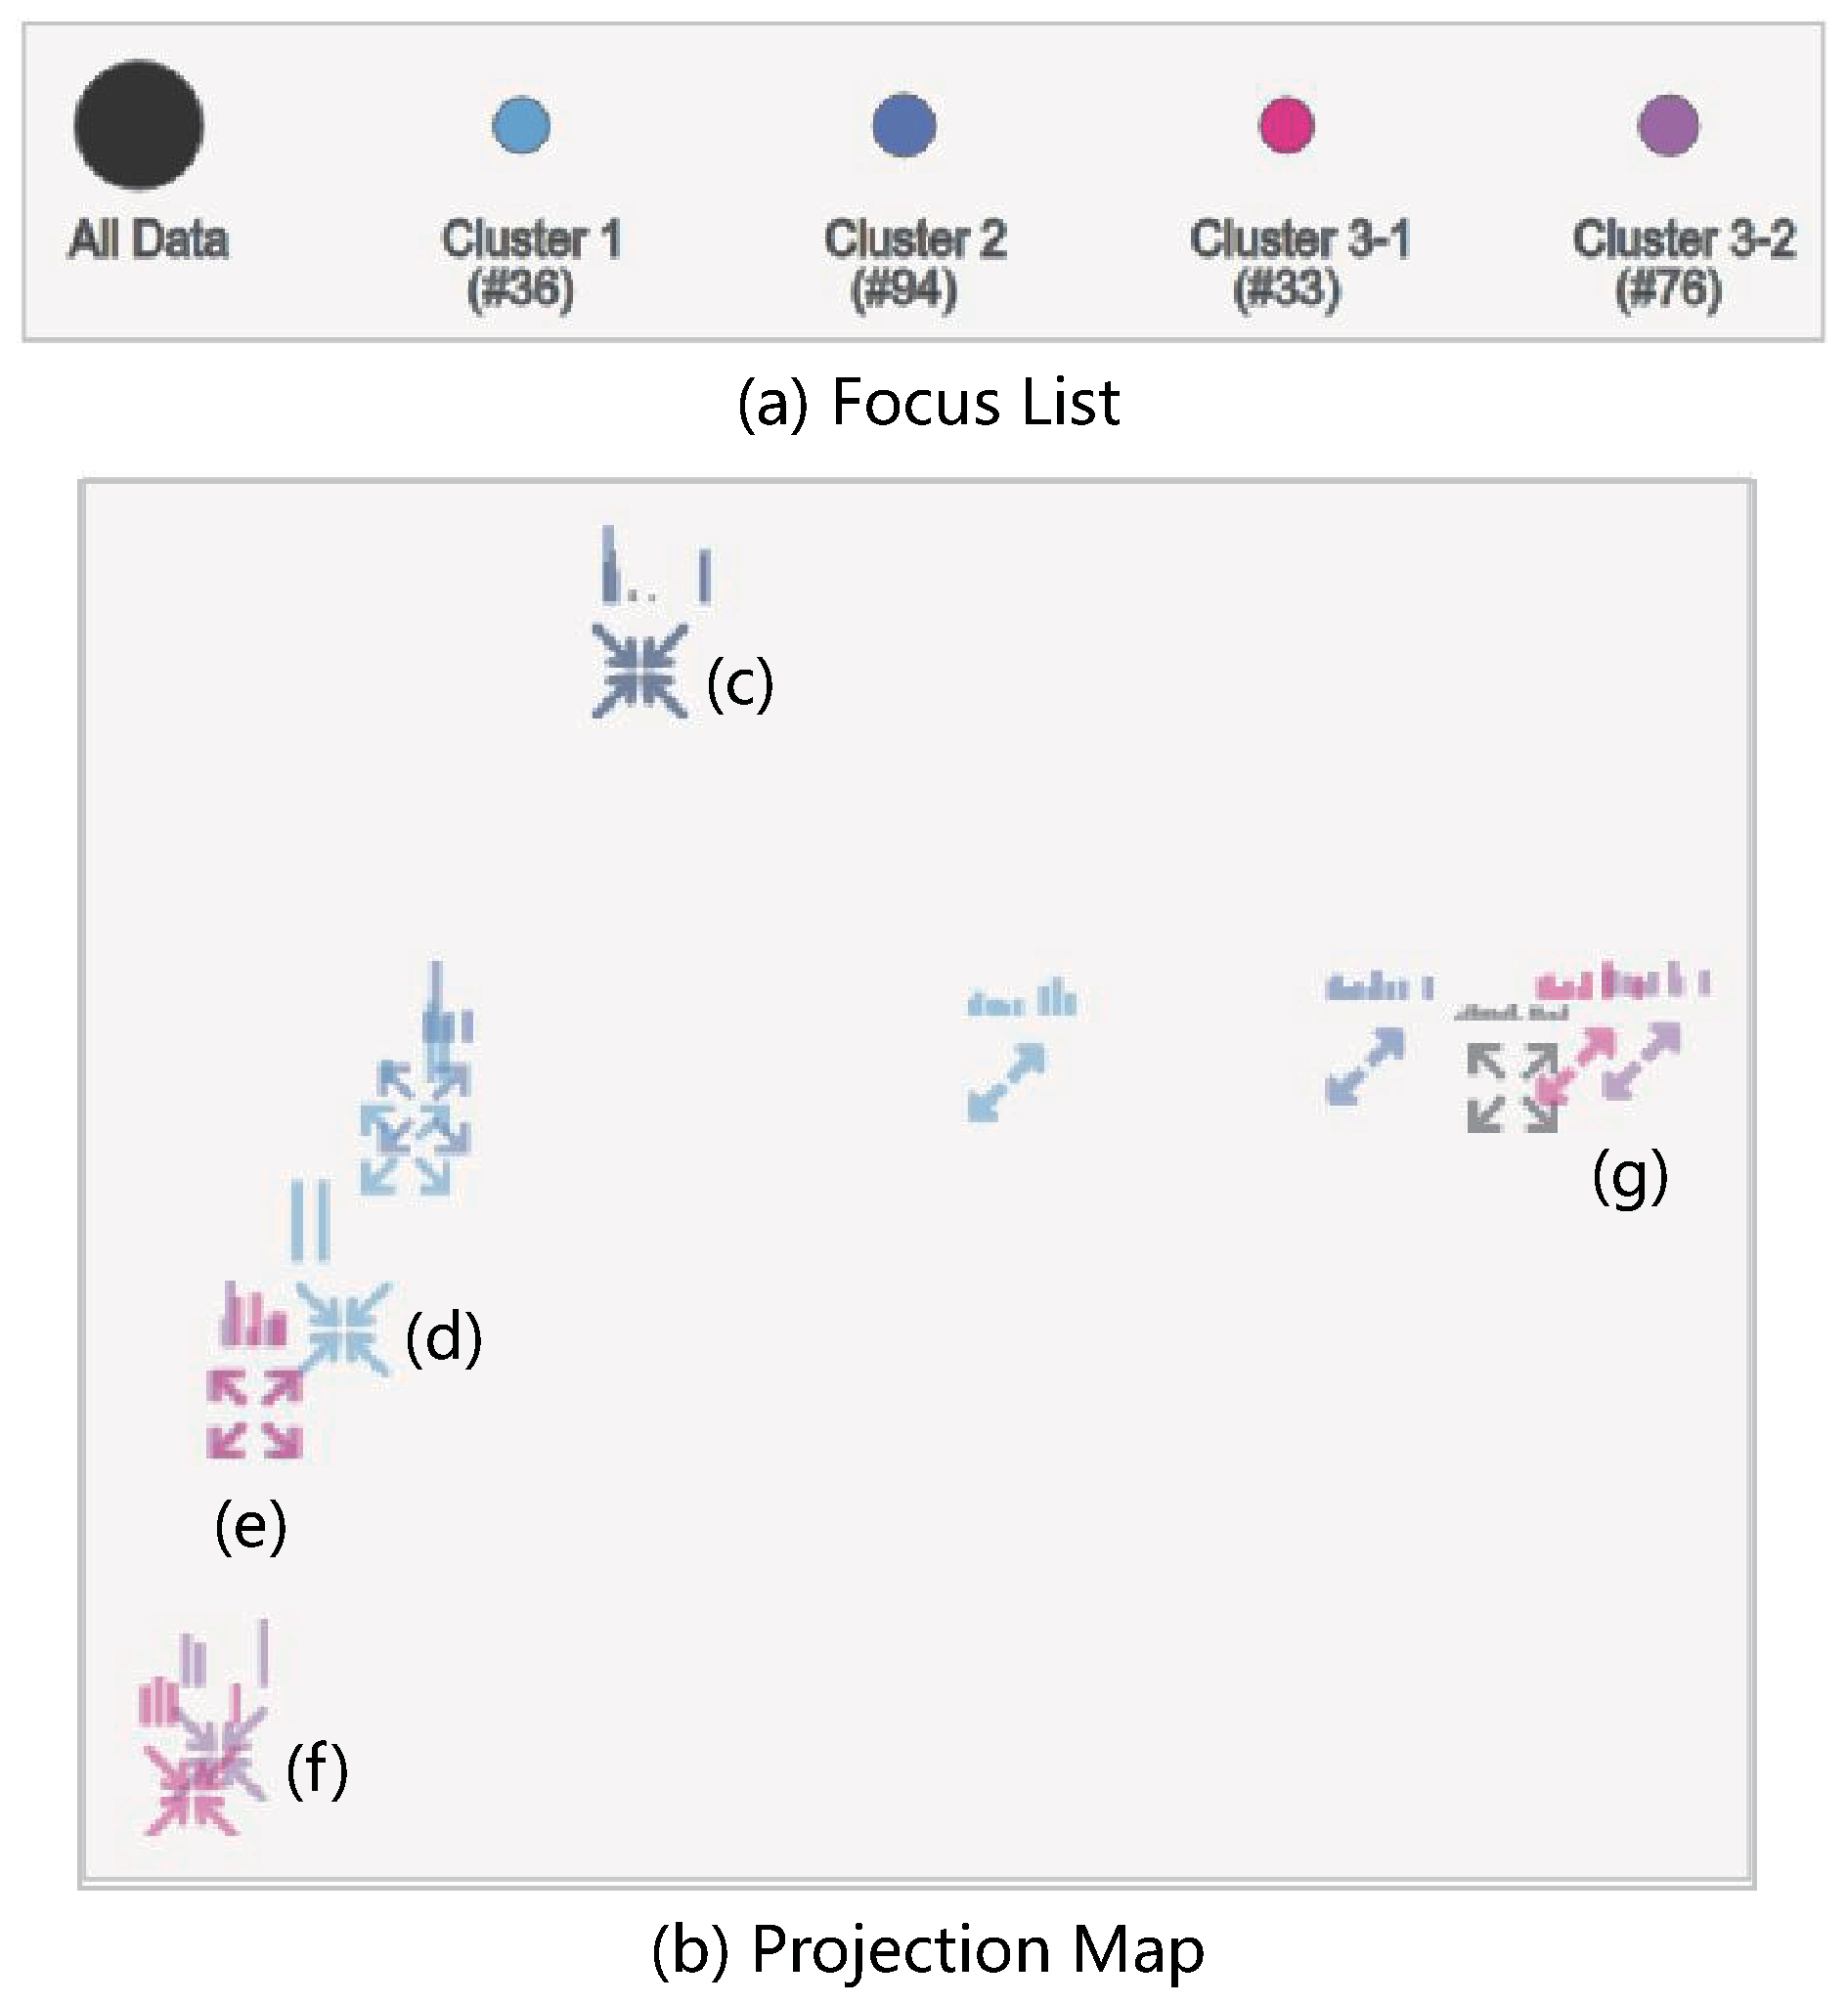
\includegraphics[width=0.85\linewidth]{images/map_2.eps}% 1\linewidth
  \caption{USDA Food Data: Four clusters found in the the exploration are stored in Focus List (a). Projection Map helps to compare them based on the featured projections. It can be seen from dimensional weights that, Compress projections of Cluster 1 and 2 are highly featured (c, d). Cluster 3-1 and 3-2 are very similar in all their projections (e, f, g).}
\label{fig:map}
  \end{figure}

In the enhanced projection (Figure~\ref{fig:food1}(b)), there seem to be some patterns, but not so obvious. Jean remembers that a proper subspace can reveal more prominent patterns. So she turns on the subspace suggestion, gaining the result in Figure~\ref{fig:food1}(c). Now she can clearly see a large cluster with several outliers. The outliers even include two tiny clusters dominating two dimensions (vitamin D and Sodium). She feels encouraged by the clear structure, and decides to go deeper.

Jean chooses the major cluster as a new focus, using the 'Decrease' brush to avoid including contextual data. She wants to know both similarities and dissimilarities among cluster members, so she applies Compress and Expand projections respectively (Figure~\ref{fig:food2}(b),(c)). The Compress view tells her that this cluster contains more water and energy than the other foods, but is poor in carbohydrate. 'Ha! They must not be gains,' she thought, 'Maybe grains are in the other two clusters'. On the other hand, data in the Expand view are separated into three sub-clusters along four dimensions, all of which are vitamins. 

She applies Compress to two sub-clusters, gaining results in Figure~\ref{fig:food2}(g) and (h). Sub-cluster 1 exhibits a very strong feature (all data gathering around the origin) that, none of its members contains fiber or beta carotene. It confirms Jean's previous guess. Sub-cluster 2 did not show much information beyond Figure~\ref{fig:food2}(c). But she notices that this sub-group is the most similar to the contextual data, as shown in the Expand view (Figure~\ref{fig:food2}(c)). 'These should be animal-based foods,' she thought, 'but cluster 1 may contain plaint-based outliers. I should check it later.' She stores the two sub-clusters in Focus List for further study, before going deeper into the last sub-cluster.

After expanding the last group, she quickly identifies a large cluster with a few outliers. She picks out the cluster and applies the enhancements. Again, no fibre or vitamin C, should be animal-based foods. But the Expand view shows two sub-groups, which surprises her:'Did I just find a local food hierarchy?' The two sub-group are mainly diverse in vitamin B6 and Sodium. She also stores them in the list.

\begin{figure*}[htbp]
\centering
  \includegraphics[width=0.97\linewidth]{images/food_1.eps}% 1\linewidth
  \caption{USDA Food Data: User chooses a global cluster as the focus (a), and enhances the projection to explore its features (b, c). Outliers can be found in the suggested subspace (d), which are hard to discern in the global projection (f).}
\label{fig:food1}
  \end{figure*}

\begin{figure*}[htbp]
\centering
  \includegraphics[width=0.97\linewidth]{images/food_2.eps}% 1\linewidth
  \caption{User focuses on the cluster found in a previous step. Similarities (b) and diversities (c) are revealed among the cluster members. Three sub-clusters are found. One of them exhibits a very strong feature that it contains no fibers of beta carotene (g). It could be a group of animal-based foods.}
\label{fig:food2}
  \end{figure*}

\begin{figure*}[htbp]
\centering
  \includegraphics[width=0.97\linewidth]{images/food_3.eps}% 1\linewidth
  \caption{User focuses on a sub-cluster found in Figure~\ref{fig:food2}(f). She gets the major group by removing a few outliers (b). This group shows a strong Compress feature (d), as well as an interesting inner structures (c). Again, two sub-clusters (e, f) are found within the focus. They seem to be small neighboring clusters in the overview (g, f).}
\label{fig:food3}
  \end{figure*}

Jean finally gets to enjoy all the trophies she've collected in the exploration. She names the stored clusters by their hierarchy, and then tries to compare them in the Projection Map (Figure~\ref{fig:map}). The map shows a very close relationship between cluster 3-1 and 3-2, in all three featured projections (Figure~\ref{fig:map}(e), (f), (g)). She also finds the strong Compress features she've met in the exploration (Figure~\ref{fig:map}(c), (d)). Hovering on each cluster allows her to highlight them in the global projection (Figure~\ref{fig:food2}(i), (j) and Figure~\ref{fig:food3}(g), (h)). Different clusters occupy different layers in the overview, which seems reasonable to her. 'It's not that hard, right?' Jean feels pleased by all the findings and insights she've got in this little exploration.

\note{
We choose one as the focus, aiming to analyze what foods it may contain. We use the Expand projection to see its inner structures (Figure~\ref{fig:food1}(b)). There seem to be some patterns, but not so obvious. We seek for the subspace suggestion with the threshold $R$ being $0.75$. The threshold keeps unchanged in the following process. Within the suggested subspace, we can see a more clear separation between a large  cluster and some outliers (Figure~\ref{fig:food1}(c)). In fact, the outliers include two tiny clusters, dominating two dimensions (vitamin D and Sodium) respectively. Turning back to the overview, we find that the outliers are scattered all over the local region (Figure~\ref{fig:food1}(f)). It's hard to recognize and remove them without a proper local projection. So far, it is the first-level local analysis.

Then we go into the large cluster (Figure~\ref{fig:food2}(a)), to study the second-level locality. The cluster is extracted from the focus using the Decrease mode. In the Compress projection (Figure~\ref{fig:food2}(c)), a three-dimensional subspace is suggested. It shows that cluster members generally contain much energy and water, but have lower carbohydrate than the others. No matter what foods they are, they are unlikely grains. The subspace gets a score of 0.88, implying that the feature is rather obvious. The Expand projection (Figure~\ref{fig:food2}(b)) has four suggested dimensions: vitamin D, vitamin B6, vitamin A and vitamin B12. The focus is divided into three smaller clusters, each dominating one or two dimensions.

The first cluster (Figure~\ref{fig:food2}(d)) scores high in vitamin D and vitamin B6. They are probably not vegetables and fruits, which are poor in vitamin D. The Compress projection (Figure~\ref{fig:food2}(g)) degrades to a 2D plane without using subspace suggestion. It's a strong pattern that none of the members has any fiber or beta carotene. This confirms our previous guess. Hence, we come to a primary conclusion: this cluster are probably fishes or dairy products, which are rich in vitamin D and vitamin B6.

The second cluster (Figure~\ref{fig:food2}(e)) scores high in vitamin A, which is a property of animal livers. But it's also relatively low in vitamin D, B6 and B12. This is a feature of plant-based foods. Most unselected data (colored in gray) behave similarly. Since the featured projection (Figure~\ref{fig:food2}(h)) did not give further information, we simply assume the cluster to be vegetables or animal livers. Back in the overview (Figure~\ref{fig:food2}(j)), these data are very close to the unselected data, which coincides with the local observation.

The third cluster seems rich in vitamin B12. We enhance its inner relationships, going down to a third-level analysis. Again, there is one big cluster with some outliers in the projection (Figure~\ref{fig:food3}(b)). We remove the outliers, and enhance similarities within the cluster. The Compress view (Figure~\ref{fig:food3}(d)) shows a strong pattern that no fiber or vitamin C exists here. The subspace score reaches 0.99. We can safely conclude that these are animal-based foods. In the Expand projection (Figure~\ref{fig:food3}(c)), five dimensions are suggested. The data are very diverse along the axis of lipid, while they separate into two groups in the other four dimensions. They are possibly fishes or red meats. In the overview, the two clusters are very close, yet separable (Figure~\ref{fig:food3}(g), (h)).

In the above process, we've found four small clusters within the initial global cluster. They are Cluster 1 (Figure~\ref{fig:food2}(g)), Cluster 2 (Figure~\ref{fig:food2}(h)), Cluster 3-1 (Figure~\ref{fig:food2}(e)) and Cluster 3-2 (Figure~\ref{fig:food2}(f)). The four clusters seem layered in the overview (Figure~\ref{fig:food2}(i), (j), Figure~\ref{fig:food3}(g), (h)). We store our findings in the focus list, and use the projection map to help compare these data (Figure~\ref{fig:map}). As shown in the map, Cluster 1 and 2 have very prominent features that are strongly related to only a few dimensions (Figure~\ref{fig:map} (c), (d)). It coordinates with findings in Figure~\ref{fig:food2}(g) and Figure~\ref{fig:food3}(d). On the other hand, Cluster 3-1 and Cluster 3-2 show close relations in the map. All three kinds projections are placed very closely (Figure~\ref{fig:map} (e), (f), (g)). It also coordinates with our previous finding that they are similar sub-clusters within Cluster 3.
}

 \note{In general, we have found outliers and hierarchical clusters in different levels of locality. Without the featured local projections or the projection map, it's hard for users to discover, interpret, and compare those clusters. In addition, such projections also help to understand the unselected data, and how the focus resembles or differs from them.}

\note{compare to histograms: easy to find the most featured dimensions}